\documentclass{beamer}
\usepackage{graphicx}
\usepackage{subcaption}
\usepackage{wrapfig}
\usepackage{setspace}
\usepackage{xcolor}
\usepackage{tabularx}
\usetheme{Madrid}
\usecolortheme{default}

\title[21G378383]{Translation / Transliteration of Vernacular Languages from Signboards}
\subtitle{Project ID:21G378383\\Review - II}
\author[SRM Institute of Science \& Technology]{Group~Members\\RA1711003030378~Vishnu~Teja~Chikkala\\RA1711003030383~Rajpreet~Srivastav\\ \medskip{Supervised By:\\Mr.~Sunil~Kumar\\Assistant~Professor}}
\institute[]{Department of Computer Science \& Engineering\\Faculty of Engineering \& Technology\\SRM Institute of Science \& Technology}
\logo{
\includegraphics[scale=.4]{srm_logo}}
%\author{Vishnu Teja Chikkala}
\date{\today}

\begin{document}
	\begin{frame}
		\maketitle
		\date{}
	\end{frame}
	\begin{frame}[allowframebreaks]{Table of Contents} %we can expand the table of contents in more than on frame
		\tableofcontents[sections={1-4}]
		\framebreak
		\tableofcontents[sections={5-8}]
	\end{frame}
	
\section{Objective}
\begin{frame}[allowframebreaks]{Objective}
\begin{itemize}
	\item India has 22 constitutionally recognized languages written in 13 different scripts. An average traveler, when travelling to a new region, might often get confused with signboards written in an unfamiliar language. It is also impossible to have every signboard in every city / town / village written in 22 different languages, as there will not be enough room to accommodate more than 2 – 3 scripts.
	\item The objective of this project is to develop a simple and easy-to-use Android mobile app which provides a two-click, picture-to-text, translation / transliteration service for Indian vernacular languages, using deep neural networks and natural language processing models trained for text detection, recognition and translation tasks on collected and freely-available datasets.
	\item For the scope of this project, we will design a system which works for names (such as road names, city names, shop names, organization names, etc.) which typically are not longer than 4-5 words, and support translation for 1 or 2 languages. Further scope for the project involves including support for more languages and building models to support translation / transliteration of longer pieces of text.
\end{itemize}
\end{frame}

\section{Summary of Literature Review}
\begin{frame}[allowframebreaks]{Summary of Literature Review}
\begin{itemize}
		\item Indian community faces a “Digital Divide” due to dominance of English as mode of communication in higher education, judiciary, corporate sector and Public administration at Central level whereas the government in states work in their respective regional languages \cite{kurian2008natural} 
		\item India has 22 scheduled languages. While 99 \%  of the population speak one of these scheduled languages in various dialects (which number in the thousands) \cite{theindianexpress_2018}, according to Census 2011, the total percentage of English speakers is at 10 \%, and that too is skewed towards the urban population. \cite{s_2019} Hence, there lies a need for developing NLP architectures for facilitating flow of digital content and information in and between local, national and international levels.
		\item The above also means that a large percentage of the literate population is either monolingual or bilingual, and across 22 languages, an accessible, easy-to-use and intuitively developed system is required, which enables intercommunication.
		\item While traditionally NLP has been approached with statistical methods such as Hidden Markov Machines (HMM), Support vector machine(SVM), Conditional Random Field(CRF), Naive Bayes(NB), etc, which take a large amount of tagged/annotated data (corpus) to statistically analyze and learn the language characteristics \cite{desai2021taxonomic}, the research into deep learning or ‘connectionist approach’ \cite{desai2021taxonomic} with the use of trained artificial neural networks (ANNs), has gained impetus due to (i) the simplicity of the solution in rapidly prototyping and establishing practically effective systems (ii) the lower cost of annotation of the training data \cite{philip2019baseline}, and the fact that they attempt to more closely emulate the learning process of biological brains, among other reasons. \cite{desai2021taxonomic}, \cite{rosca2016sequence}, \cite{deselaers2009deep}
		\item Particularly, the collection of a uniform corpus and standard datasets for training models remains a challenge across all regional languages. The large number of morphological variations across Indic languages also contributes to this issue.\cite{kunchukuttan2020ai4bharat}, \cite{singhnlp}
		\item  Sharma et al., 2017 concluded that almost all  existing Indian language machine transliteration systems are based on statistical and hybrid approach \cite{sharma2017machine}
		\item Kulkarni et al., achieved upto 98\%  training and 94\% testing accuracy on the IndicNLP library for Marathi, using an CNN-LSTM based model architecture. \cite{kulkarni2021experimental}
		\item Most of the Indian population accesses digital content through smartphones. In 2019, the number of smartphone users in the country passed 500 million \cite{news18_2020}, and is estimated to increase to 850 million by 2022 \cite{www.ettelecom.com_2020}. This, hence, also makes smartphones and smartphone apps in particular an ideal platform on which to launch NLP applications for the wider population, and directly help facilitate flow of information past language barriers.
\end{itemize} 
\end{frame}

\section{Architectural Design for Proposed System}
	\begin{frame}[allowframebreaks]{Architectural Design}
	\begin{itemize}
		\item The basic functioning of the app is as follows:
		\begin{itemize}
			\item User captures a photo of the signboard
			\item The image is resized so as to be suitable as input to the model
			\item The model takes the image as input. The text within the message is detected, extracted and transcribed to target language.
			\item The text output (or error message, in case of failure to generate output within threshold confidence), is displayed on screen.
		\end{itemize}
		 \begin{figure}
				{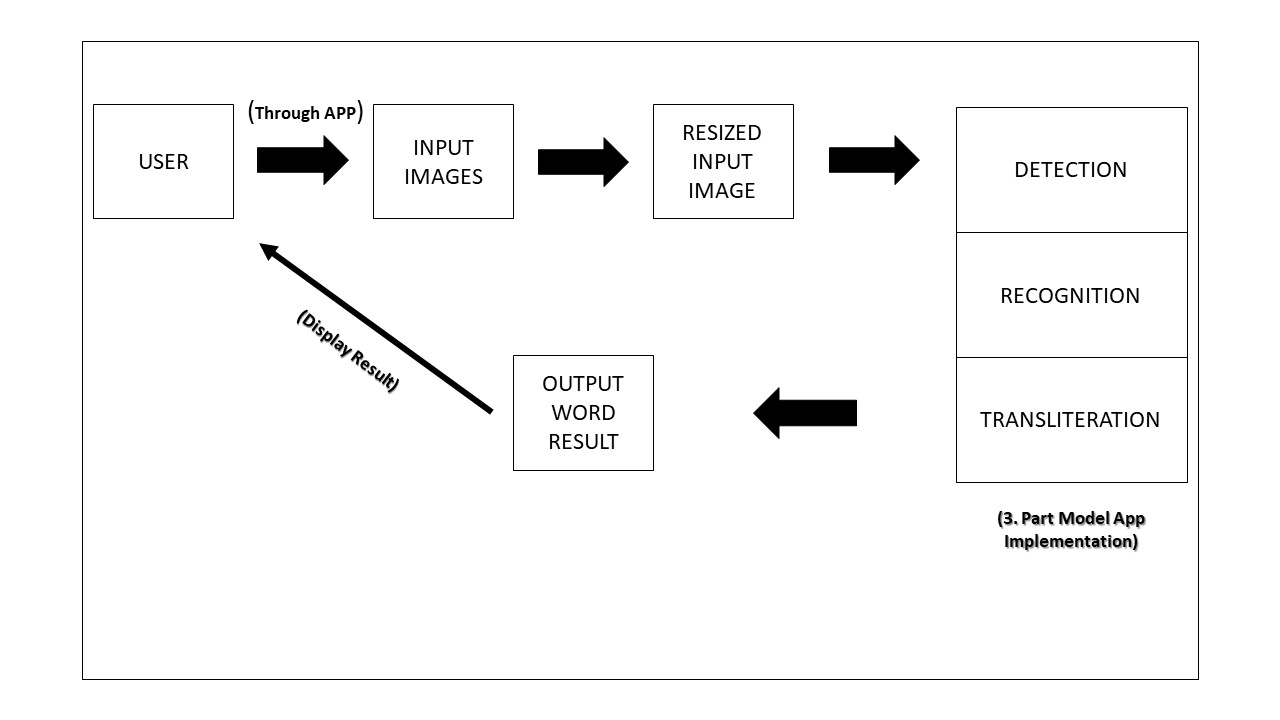
\includegraphics[scale=.3]{Slide2}}
				\caption{Functioning of App}
				\label{Slide2}
		\end{figure}
		\item The artificial neural network (ANN) behind the core functioning of the app is made up of 3 models performing consecutive tasks. That is, the output of a preceding model will be fed as input to the succeeding model, and thus they act as one model unit.
		\begin{figure}
				{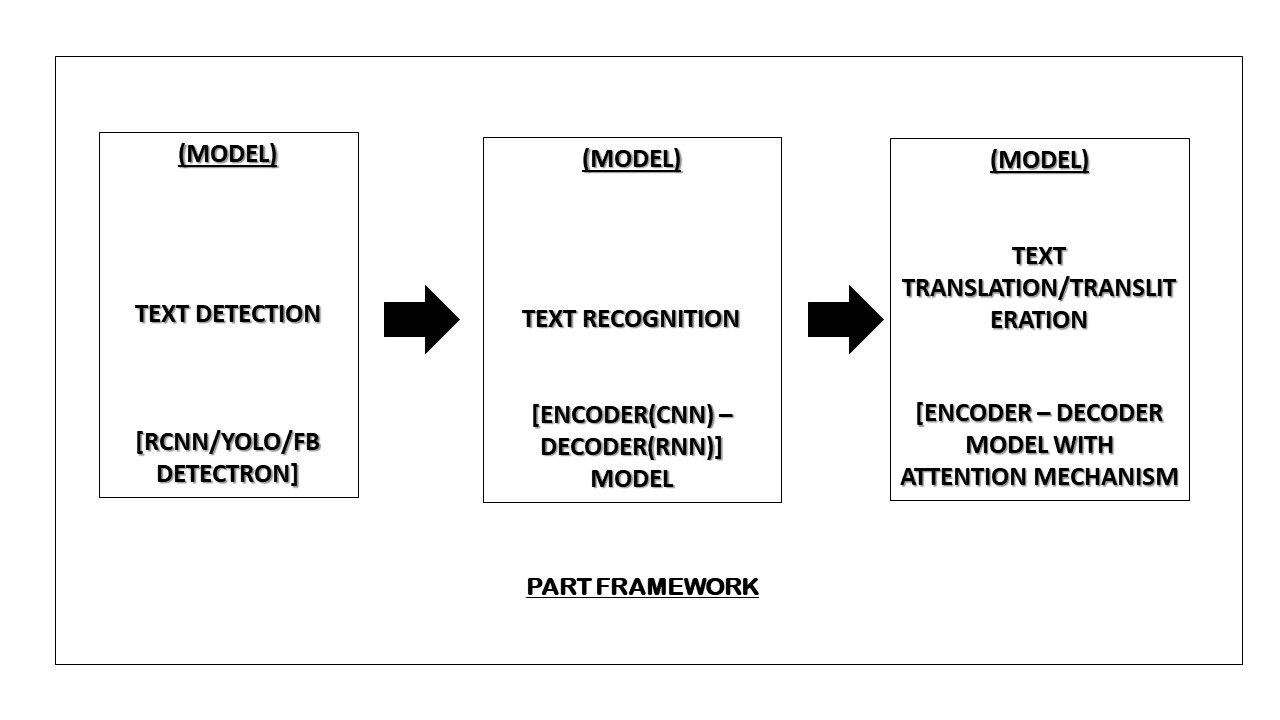
\includegraphics[scale=.3]{Slide1}}
				\caption{3-part model}
				\label{Slide1}
		\end{figure}
	\end{itemize}
\end{frame}

\section{Dataset Specifications}
\begin{frame}[allowframebreaks]{Dataset Specification}
\begin{itemize}
	\item The training dataset for the text detection and text recognition tasks consists of a large number of images containing scene text, synthetically generated. Each of the images has a corresponding annotation, listing the bounding boxes and text script present in the images.
	\begin{figure}
           \begin{subfigure}[b]{0.2\linewidth}
			{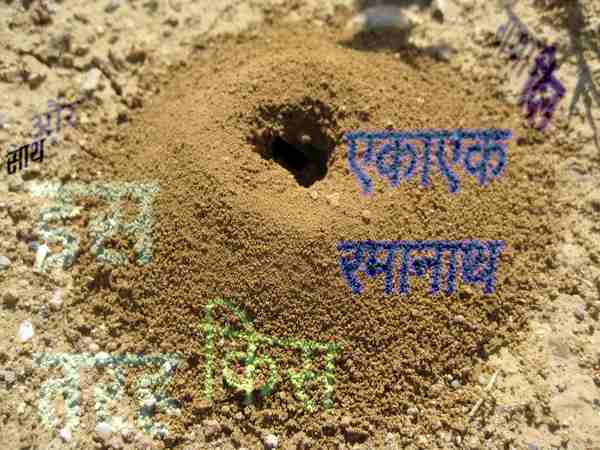
\includegraphics[width=\linewidth]{Train_Dataset_1}}
			\caption{Training Set Image}
			\label{Train_Image}
	\end{subfigure}
	\begin{subfigure}[b]{0.2\linewidth}
			{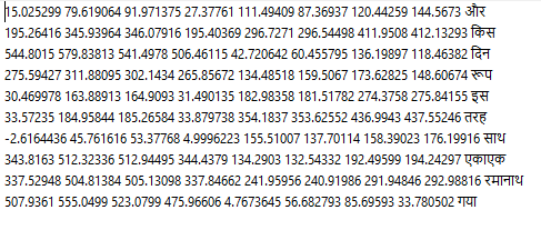
\includegraphics[width=\linewidth]{Train_Dataset_2}}
			\caption{Set Annotation}
			\label{Annotation}
           \end{subfigure}
	\end{figure}
	\framebreak
	\item  The test dataset for text detection and text recognition tasks consists of actual images containing natural scene text.
	\begin{figure}
			{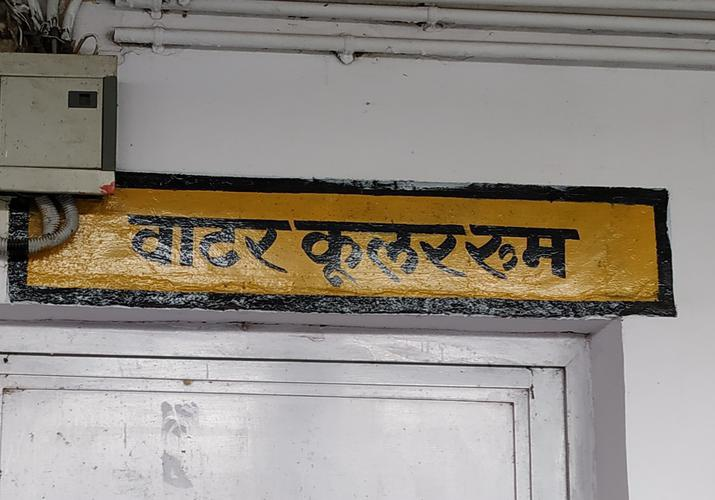
\includegraphics[scale=.3]{Test_Dataset}}
			\caption{Test Set Image}
			\label{Test_Image}
	\end{figure}
	\framebreak
	\item The train and test datasets are both in form of xml files containing serialized pairs of source language script and corresponding target language script.
	\begin{figure}
			{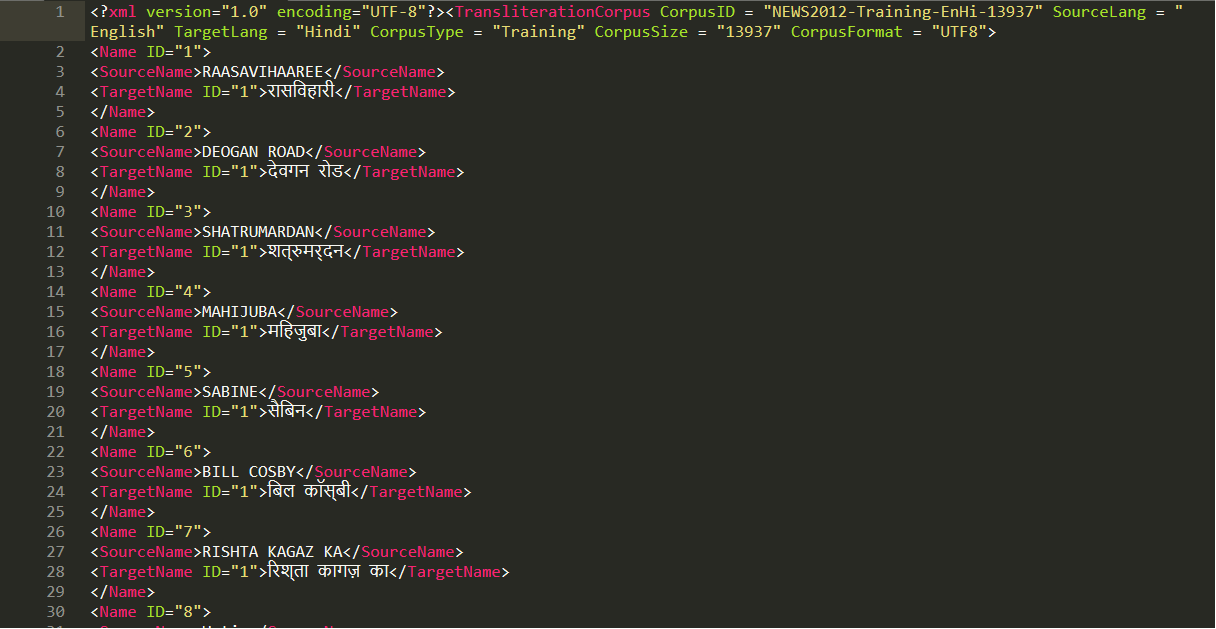
\includegraphics[scale=.3]{Transliteration_Dataset}}
			\caption{Transliteration Set}
			\label{Transliteration_Set}
	\end{figure}
\end{itemize}
\end{frame}

\section{Methodology / Algorithms / Techniques to be used}
\begin{frame}[allowframebreaks]{Methodology / Algorithms / Techniques to be used}
\begin{itemize}
	\item The text detection task will be carried out by a Faster Region-based Convolutional Network (Faster R-CNN) with Feature Pyramid Network (FPN; for bounding box tightening) from the FAIR Detectron2 kit, which has been trained for object detection on the COCO dataset. We will fine-tune this model to the task at hand by training and validating further on the above scene text database.
	\begin{figure}
			{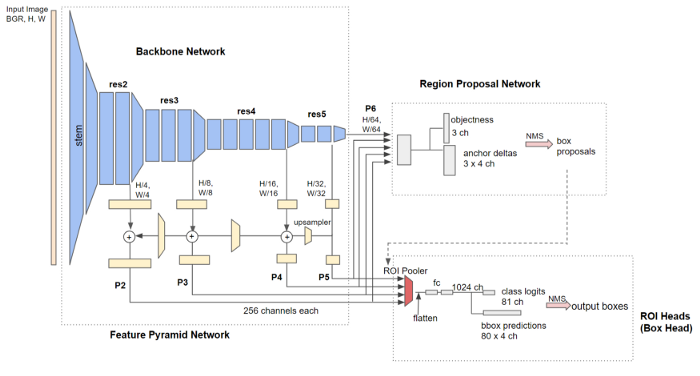
\includegraphics[scale=.4]{Text_Detection_Model}}
			\caption{Faster R-CNN Object Detection Model}
			\label{Text_Detection_Model}
	\end{figure}
	\framebreak
	\item The text recognition task will be carried out by an encoder-decoder model setup which takes the cropped bounding box of text as input. The encoder is a Convolutional Neural Network (CNN) while the decoder is a Long Short-Term Memory model (LSTM). Connectionist Temporal Classification (CTC) loss will be used to eliminate duplicate recognition of the same letter by adjacent CNN features.
	\begin{figure}
			{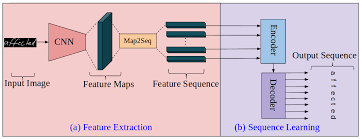
\includegraphics[scale=.6]{Text_Recognition_Model}}
			\caption{CNN-LSTM Encoder-Decoder Architecture}
			\label{Text_Recognition_Model}
	\end{figure}
	\framebreak
	\item The transliteration task will carried by a LSTM - LSTM encoder-decoder model with attention mechanism, which takes source language script as input and generates target language script as output.
	\begin{figure}
			{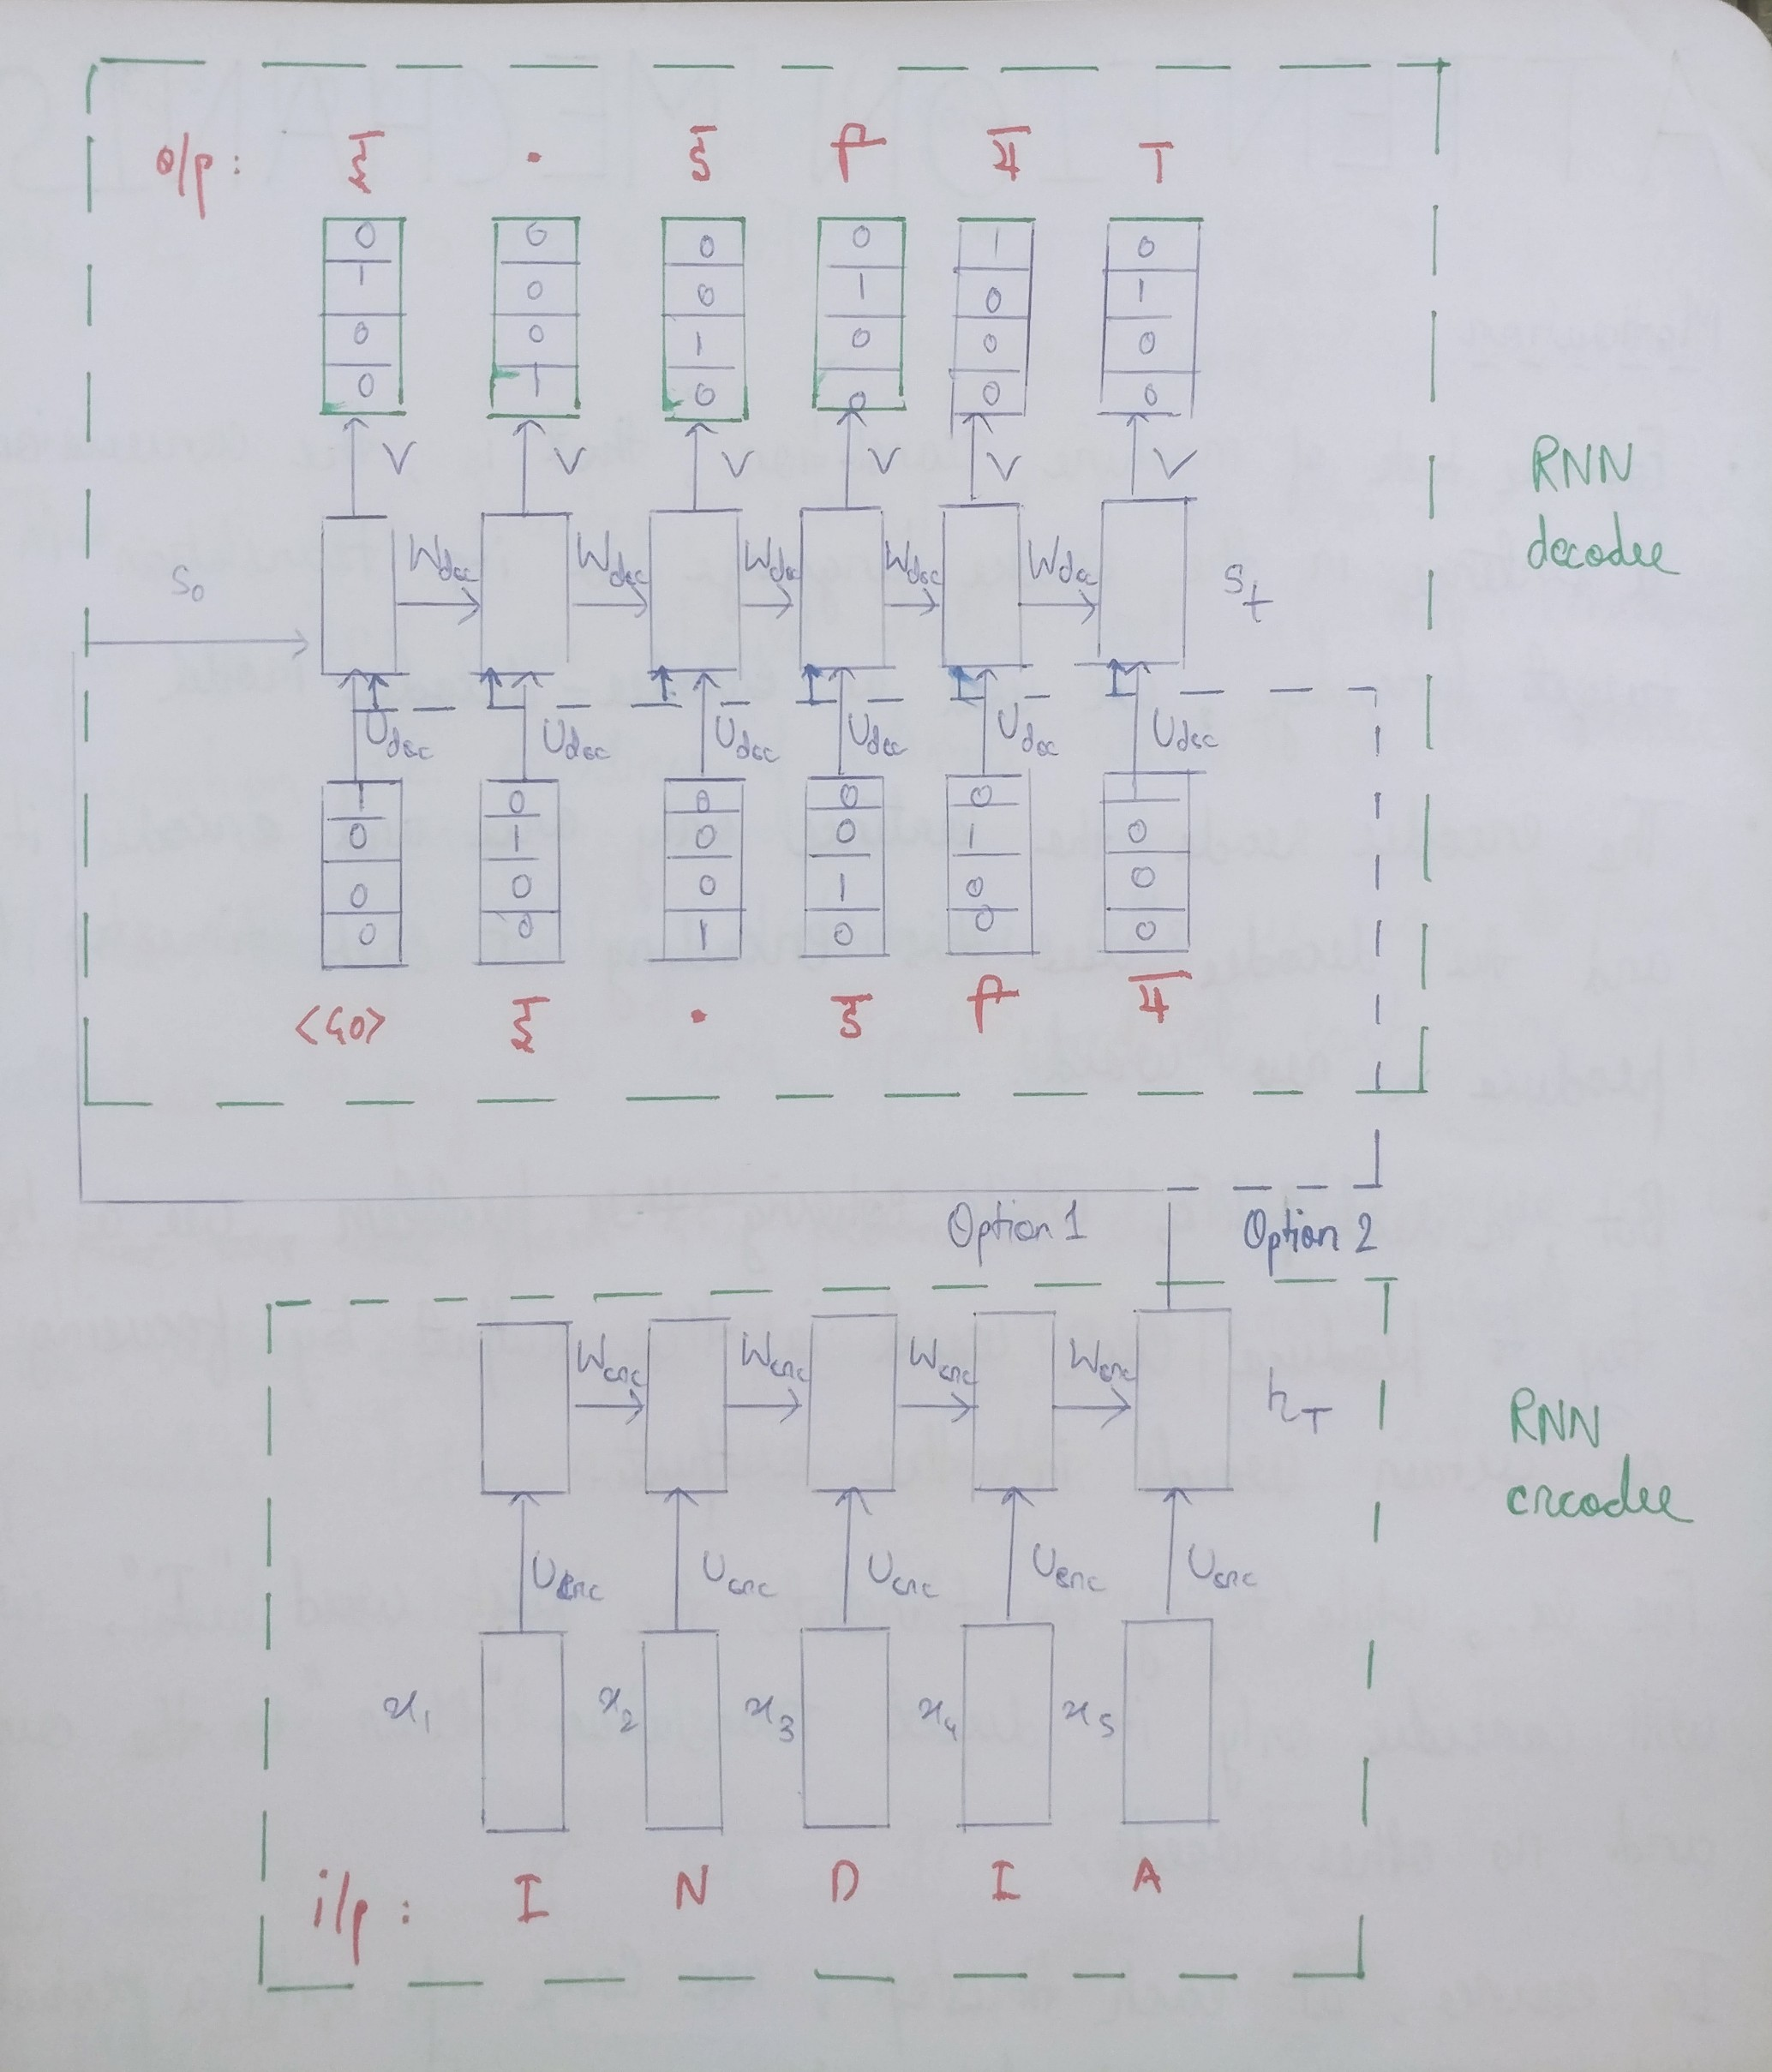
\includegraphics[scale=.05]{Text_Transliteration_Model}}
			\caption{LSTM-LSTM Encoder-Decoder Architecture}
			\label{Text_Transliteration_Model}
	\end{figure}
	\framebreak
	\item The app will make use of Google Firebase API to provide UI functionality and user services.
	\item The model will be mounted on and integrated with the app with the help of Tenserflow Lite.
\end{itemize}
\end{frame}

\section{Partial Implementation}
\begin{frame}[allowframebreaks]{Partial Implementation}
	\begin{figure}
           \begin{subfigure}[b]{0.2\linewidth}
			{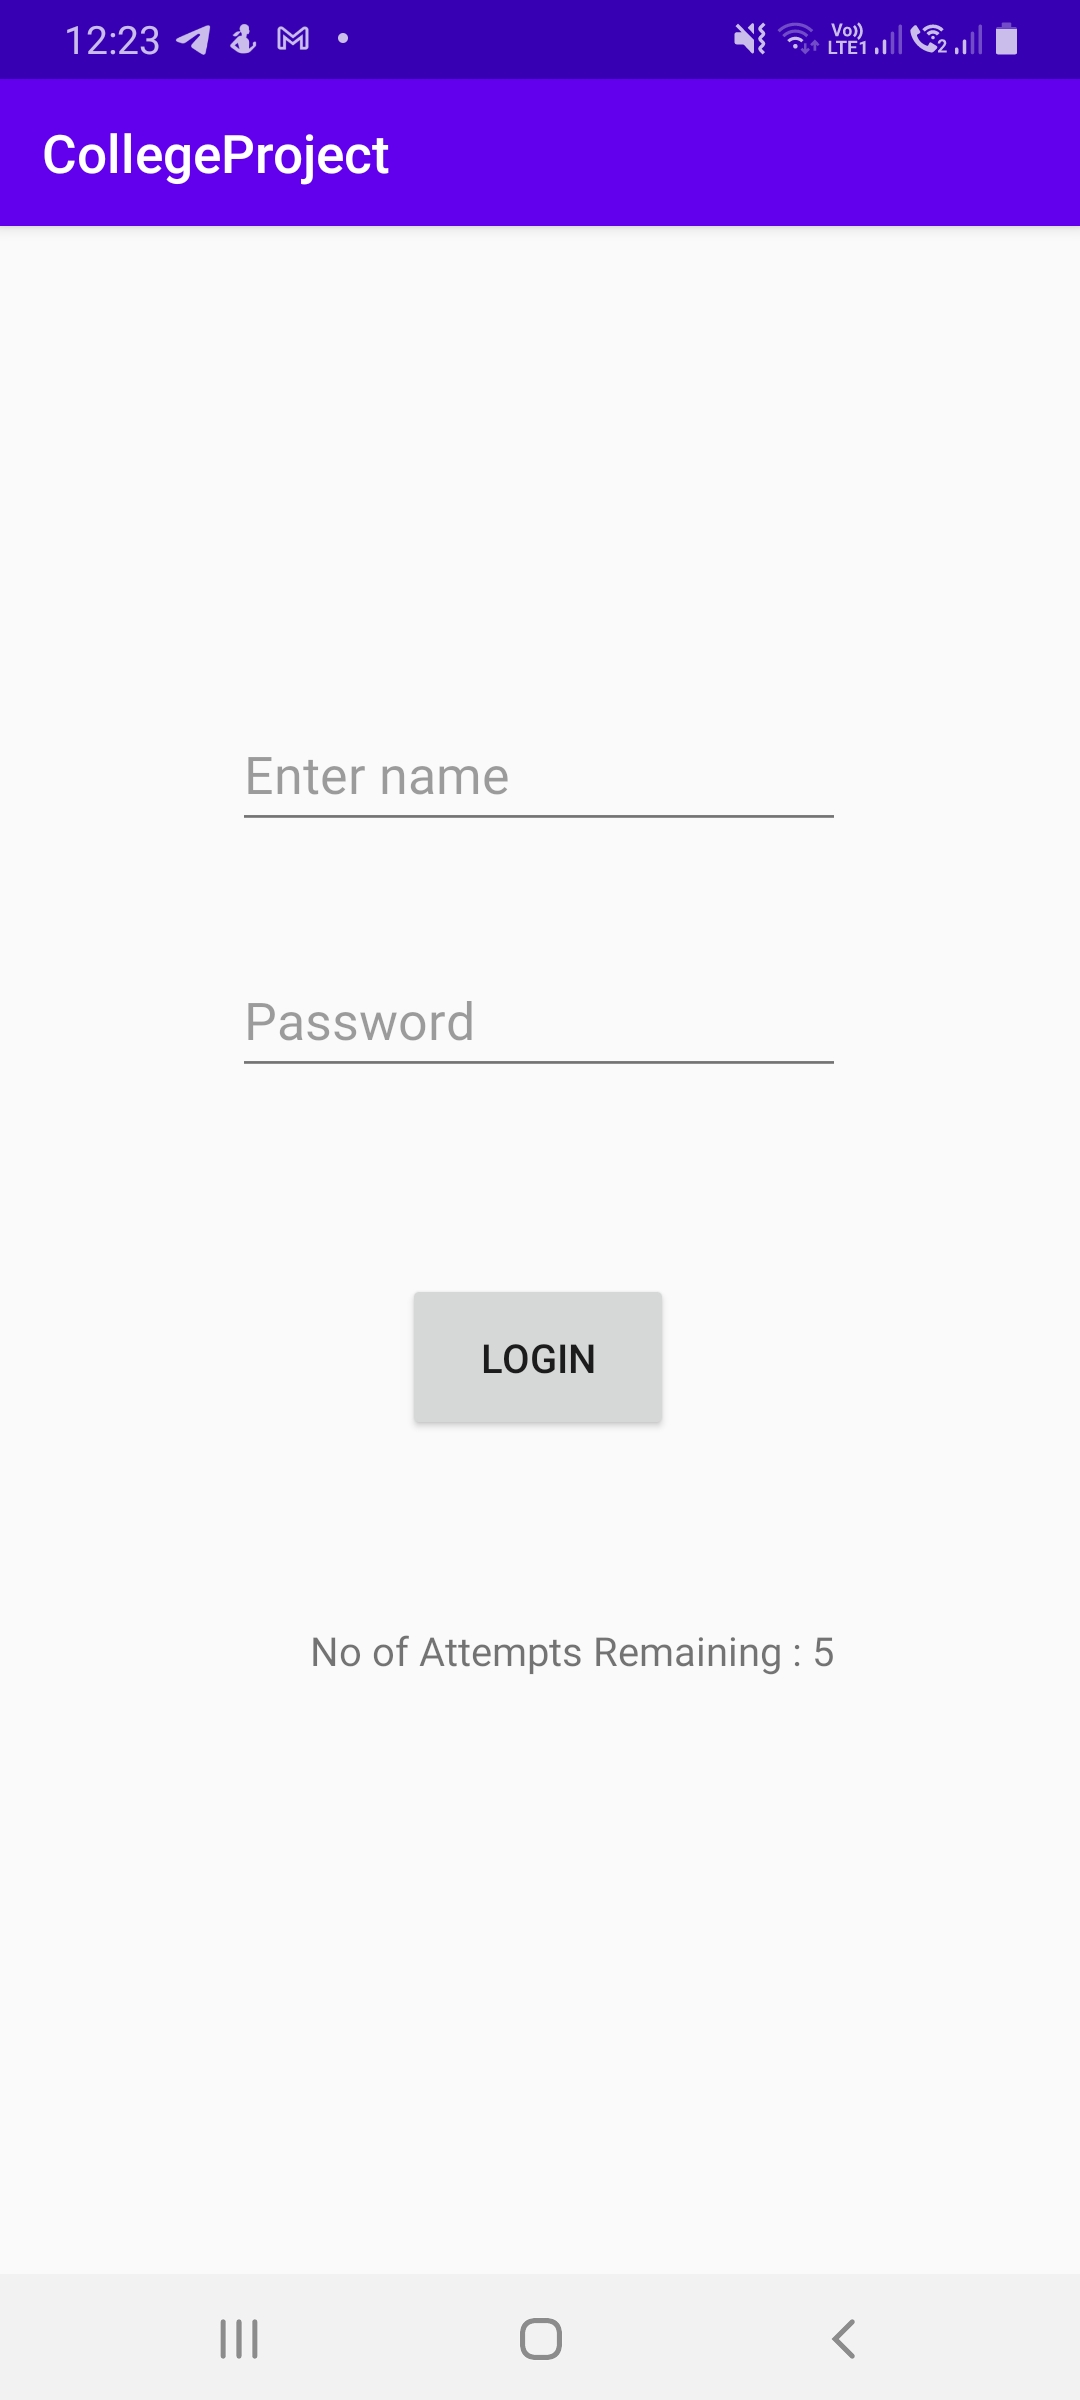
\includegraphics[width=\linewidth]{App_1}}
			\label{App}
	\end{subfigure}
	\begin{subfigure}[b]{0.2\linewidth}
			{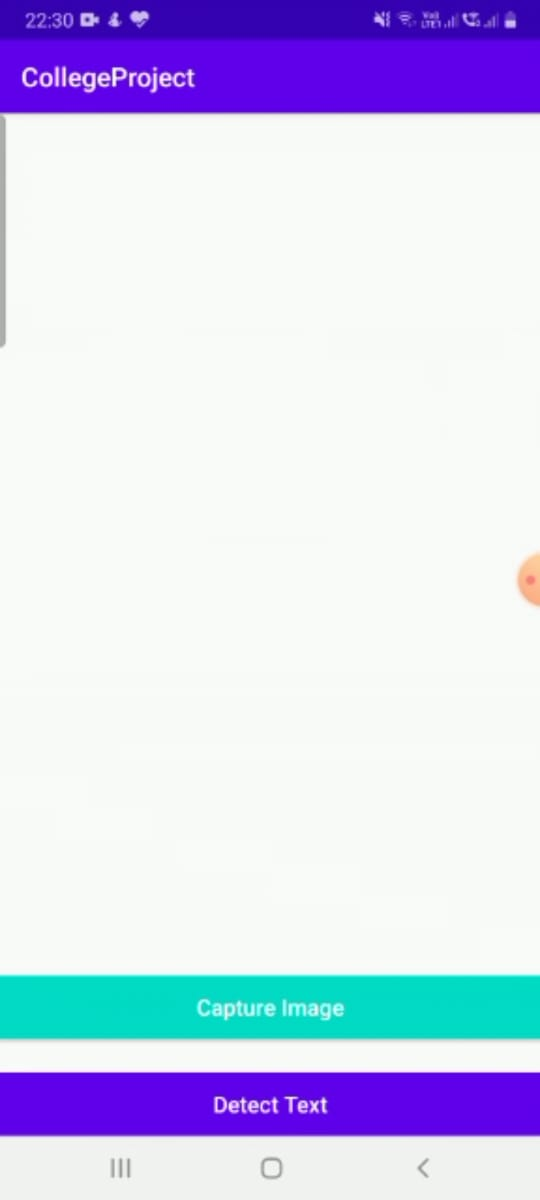
\includegraphics[width=\linewidth]{App_2}}
			\label{App}
           \end{subfigure}
	\begin{subfigure}[b]{0.2\linewidth}
			{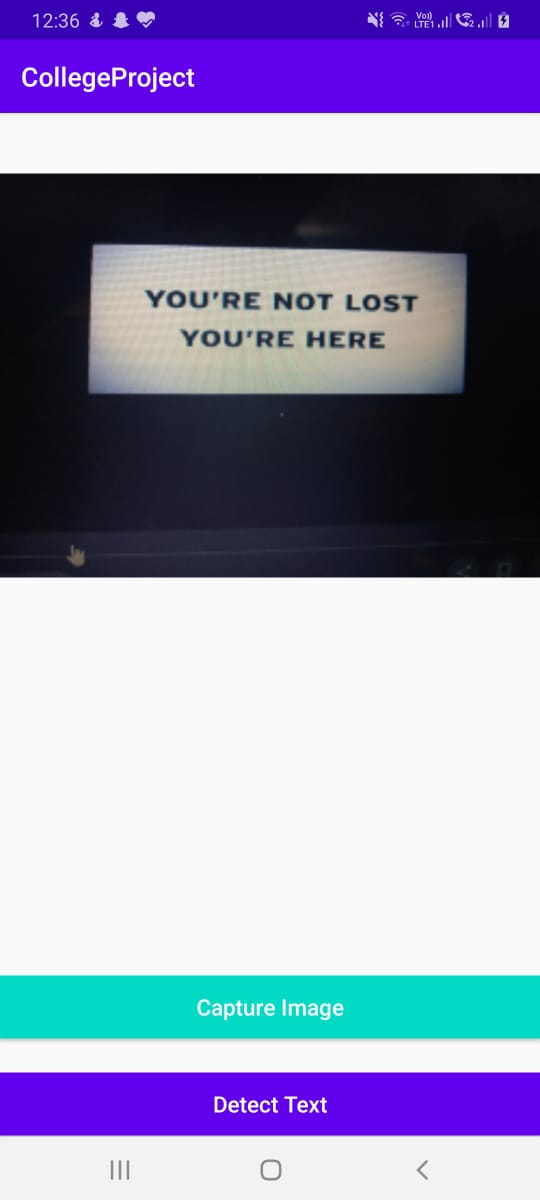
\includegraphics[width=\linewidth]{App_3}}
			\label{App}
           \end{subfigure}
	\caption{Skeleton App}
	\end{figure}
	\framebreak
	\begin{figure}
				{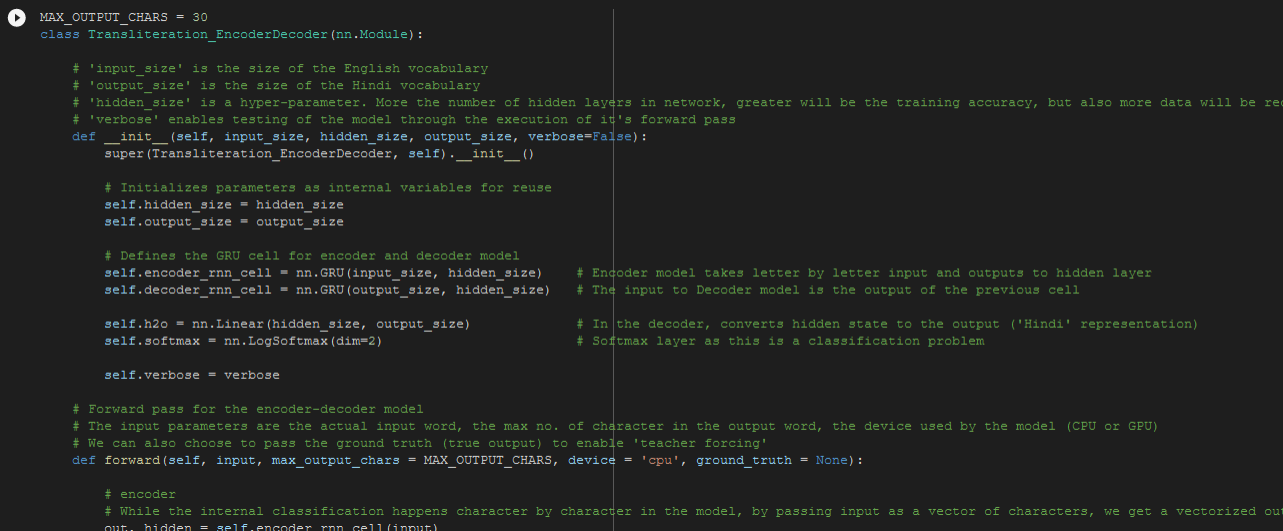
\includegraphics[scale=.3]{Translit_Model_1}}
				\caption{Text Transliteration Model}
				\label{Translit_Model_1}
	\end{figure}
	\begin{figure}
				{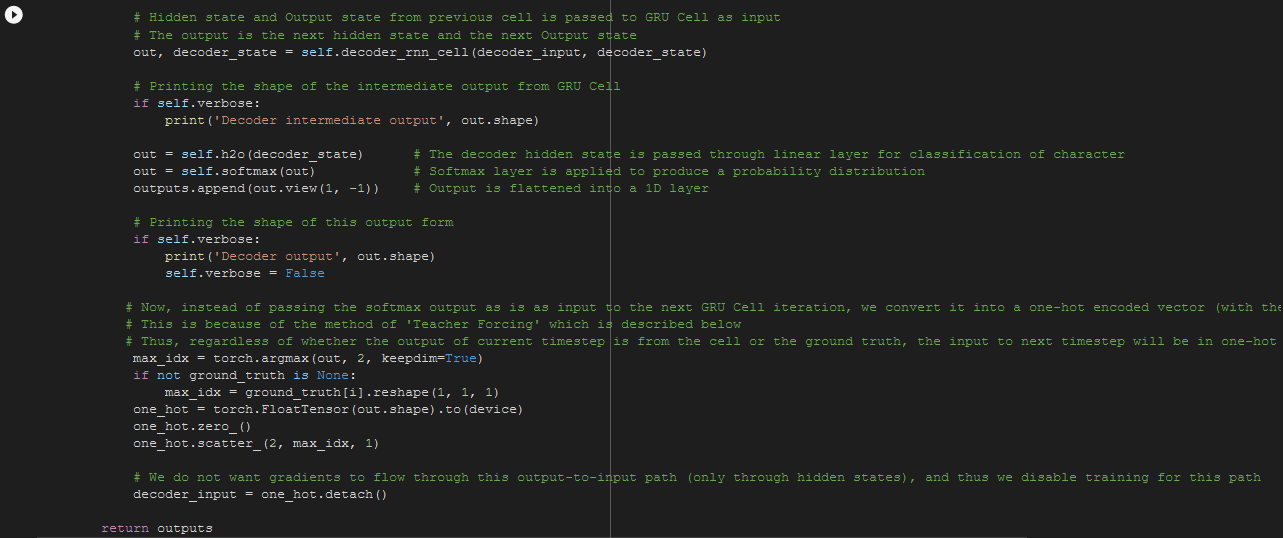
\includegraphics[scale=.3]{Translit_Model_2}}
				\caption{Text Transliteration Training}
				\label{Translit_Model_1}
	\end{figure}
\end{frame}

\section{Expected Outcomes}
\begin{frame}[allowframebreaks]{Expected Outcomes}
\begin{itemize}
\item Achieve greater than 80 \% accuracy on both train and validation / test datasets, across all models, after training, with optimal bias-variance tradeoff and set of tuned hyperparameters.
\item Propose general scalable and upgradable framework to similarly train model on other Indian languages / scripts as well as on longer pieces of text. 
\item Optimize the performance of the app w.r.t. model, to deliver seamless user experience.
\item Design app to be intuitive, easy-to-use and non-dependent on the internet.
\end{itemize} 
\end{frame}

\section{References}
\begin{frame}[allowframebreaks]{References}
	\bibliographystyle {abbrv}
	\bibliography {cite}
\end{frame}

\begin{frame}
	\begin{center}
	\LARGE
	\textcolor{red}{Thank You}
	\end{center}
\end{frame}

\end{document}